% !TeX document-id = {31cec06c-209e-42c6-b48d-393b1a0af1d2}
% !TeX TS-program = xelatex
% !BIB TS-program = biber
% !TeX encoding = UTF-8
% !TeX spellcheck = en_US
% !TeX root = seminar_presentation__intelligent_industrial_robots.tex


%% LaTeX-Beamer template for KIT design
%% by Erik Burger, Christian Hammer
%% title picture by Klaus Krogmann
%%
%% version 2.1
%%
%% mostly compatible to KIT corporate design v2.0
%% http://intranet.kit.edu/gestaltungsrichtlinien.php
%%
%% Problems, bugs and comments to
%% burger@kit.edu

\documentclass[18pt]{beamer}

\usepackage[utf8]{inputenc}

%% SLIDE FORMAT

% use 'beamerthemekit' for standard 4:3 ratio
% for widescreen slides (16:9), use 'beamerthemekitwide'
% for widescreen slide without sidebar use 'beamerthemekitwidenosidebar'

%\usepackage{templates/beamerthemekit}
%\usepackage{templates/beamerthemekitwide}
\usepackage{templates/beamerthemekitwidenosidebar}

% use this to disable the latex beamer navigation symbols
%\beamertemplatenavigationsymbolsempty


%% TITLE PICTURE

% if a custom picture is to be used on the title page, copy it into the 'logos'
% directory, in the line below, replace 'mypicture' with the 
% filename (without extension) and uncomment the following line
% (picture proportions: 63 : 20 for standard, 169 : 40 for wide
% *.eps format if you use latex+dvips+ps2pdf, 
% *.jpg/*.png/*.pdf if you use pdflatex)

\titleimage{plc_logo}

%% TITLE LOGO

% for a custom logo on the front page, copy your file into the 'logos'
% directory, insert the filename in the line below and uncomment it

\titlelogo{iar_iirob}

% (*.eps format if you use latex+dvips+ps2pdf,
% *.jpg/*.png/*.pdf if you use pdflatex)

%% TikZ INTEGRATION

% use these packages for PCM symbols and UML classes
\usepackage{templates/tikzkit}
\usepackage{templates/tikzuml}

\usepackage{tabularx}
\usepackage{multirow}
\usepackage{multicol}
\usepackage{booktabs}

\usepackage{glossaries}
\usepackage{acronym}
\usepackage{listings}

% the presentation starts here

\title[Automated Programming of Programmable Logic Controllers]{Seminar Intelligent Industrial Robots}
\subtitle{Automated Programming of Programmable Logic Controllers}
\author{David Oberacker}

\institute{
	Institute for Anthropomatics and Robotics - Intelligent Process Automation and Robotics Lab (IAR-IPR)
}

% Bibliography

\usepackage[citestyle=authoryear,bibstyle=numeric,hyperref,backend=biber]{biblatex}
\addbibresource{presentation.bib}
\bibhang1em

\newacronym{acn:PLC}{PLC}{Programmable Logic Controller}
\newacronym{acn:UML}{UML}{Unified Modeling Language}
\newacronym{acn:SysML}{SysML}{Systems Modeling Language}

\makeglossaries

\begin{document}

% change the following line to "ngerman" for German style date and logos
\selectlanguage{english}

%title page
\begin{frame}
\titlepage
\end{frame}

%\begin{frame}{Introduction}
%    \begin{figure}
%        \centering
%        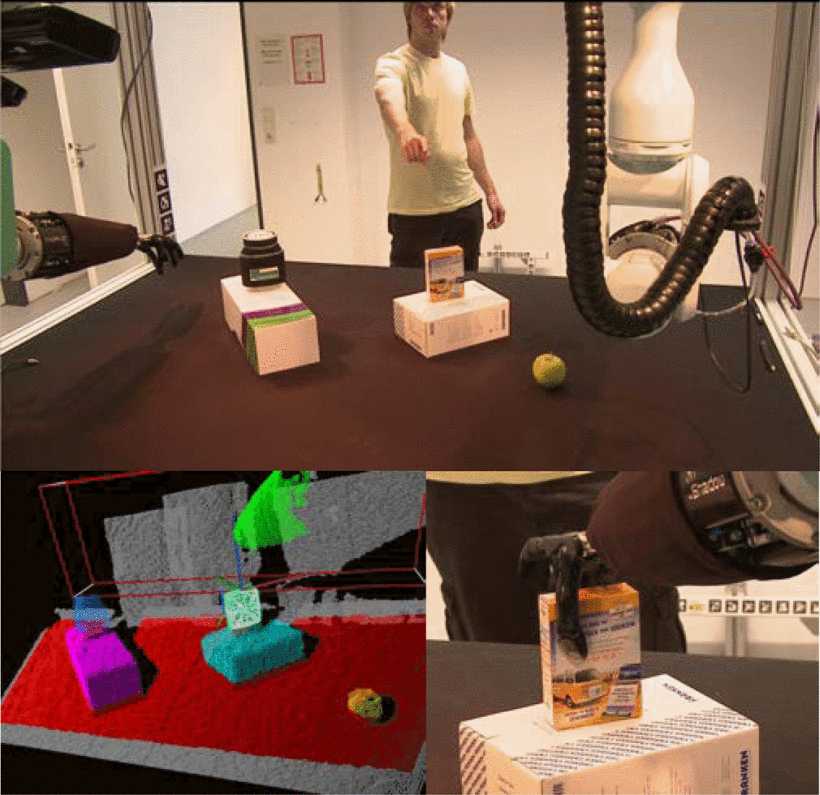
\includegraphics[height=0.7\textheight]{figures/3d_semantic_grasping.png}
%    \end{figure}
%\footcitetext{6385692}
%\end{frame}

%table of contents
\begin{frame}{Outline}
\tableofcontents
\end{frame}

\section{Introduction}

\begin{frame}{Introduction}
    
    \begin{itemize}
        \item Automation is a important factor in todays industry.
        \item With Industry 4.0 automation systems have to get more flexible.
        \item Common controller in automation are~\acrfull{acn:PLC}.
        \item They are programmed in a static and non-flexible manner.
    \end{itemize}
	\pause
    $\Rightarrow $ Are there ways to program a~\acrshort{acn:PLC} in a more flexible way ?
    
\end{frame}

\section{Programmable logic controller}

\begin{frame}{Programmable Logic Controller}
\begin{columns}
    \begin{column}{0.5\textwidth}
        \begin{itemize}
            \item Specialized industrial computers.
            \item Fixed~\textbf{cycle based} execution semantic:
            \begin{enumerate}
                \item Copy~\textbf{input} variables values from the physical interfaces to the RAM.
                \item \textbf{Execution} of the~\textbf{user program}.
                \item Copy~\textbf{output} variable values from the RAM to the physical interfaces.
            \end{enumerate}
            \item Programmed via the languages defined in the IEC 61131-3 standard.
        \end{itemize}
    \end{column}
    \begin{column}{0.5\textwidth}
        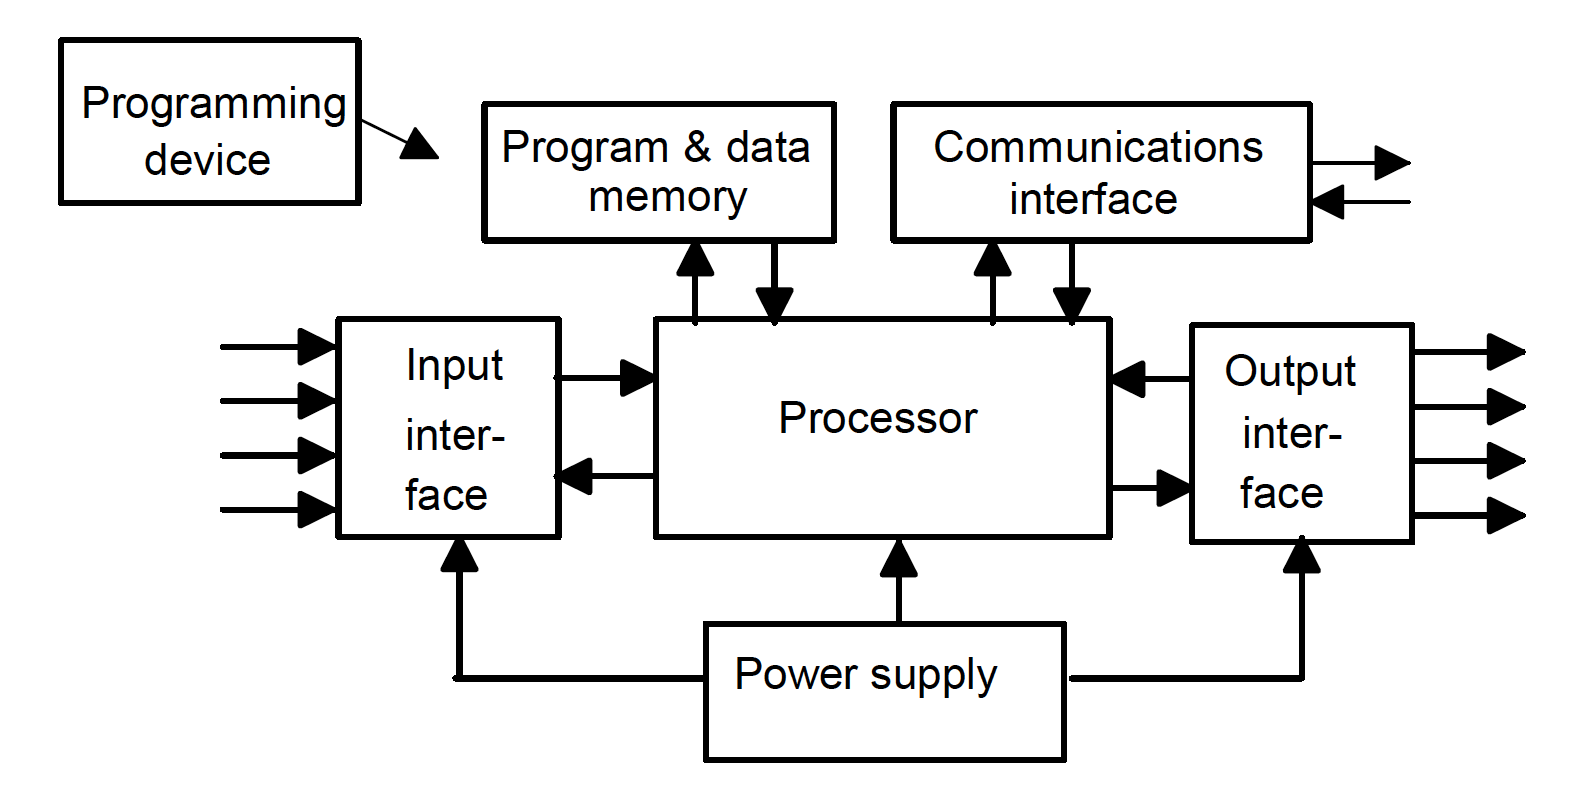
\includegraphics[width=\textwidth]{figures/PLC_Architecture.png}
        {\footnotesize Source:~\cite{BOLTON200653}}
    \end{column}
\end{columns}
\end{frame}

\subsection{IEC 61131-3 Languages}

\begin{frame}{Ladder Diagram}
\begin{columns}
	\begin{column}{0.5\textwidth}
		\begin{itemize}
            \item Graphical programming language.
            \item Historical importance.
			\item Similar to electrical relay diagrams.
			\item The named contacts are inputs, outputs and state variables.
			\item Can be combined with different operators (e.g. Not, $ >$, etc.).
		\end{itemize}
	\end{column}
	\begin{column}{0.5\textwidth}
		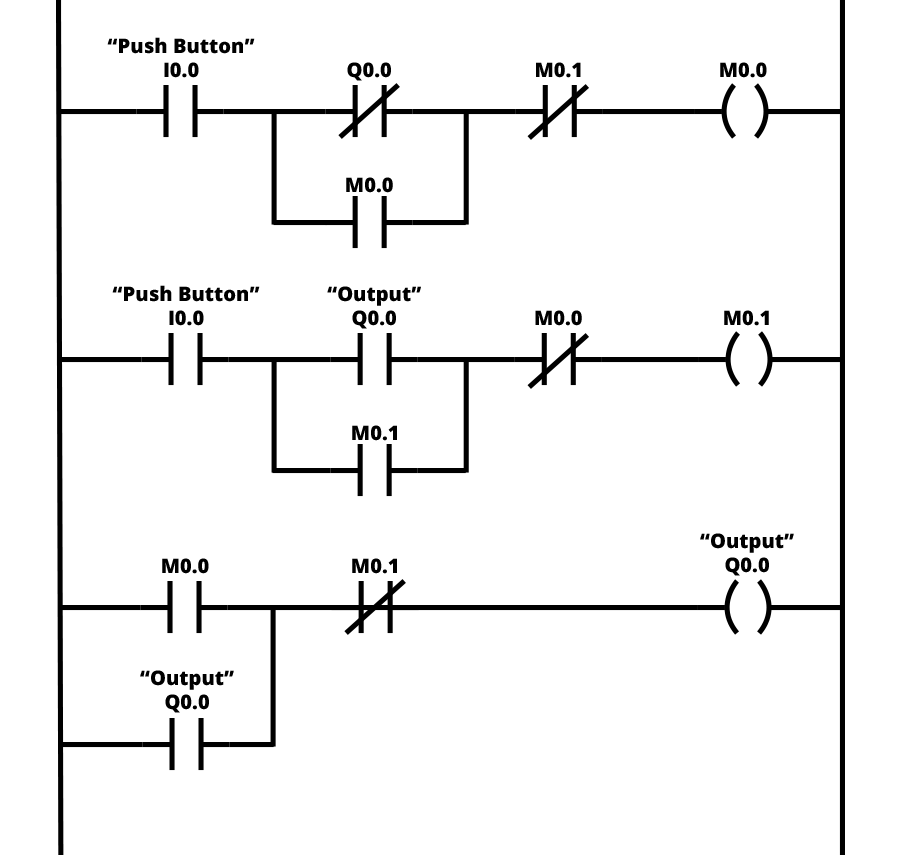
\includegraphics[width=0.8\textwidth]{figures/ld.png}
       {\footnotesize  Source:~\url{https://www.plcacademy.com/ladder-logic-examples/}}
	\end{column}
\end{columns}
\end{frame}

\begin{frame}[fragile]{Structured Text}
    \begin{columns}
        \begin{column}{0.5\textwidth}
           \begin{itemize}
               \item Textual programming language.
               \item Syntax is similar to PASCAL.
               \item Allows for more complex control flows.
               \item Currently the most used IEC 61131-3 language.
           \end{itemize}
        \end{column}
        \begin{column}{0.5\textwidth}
            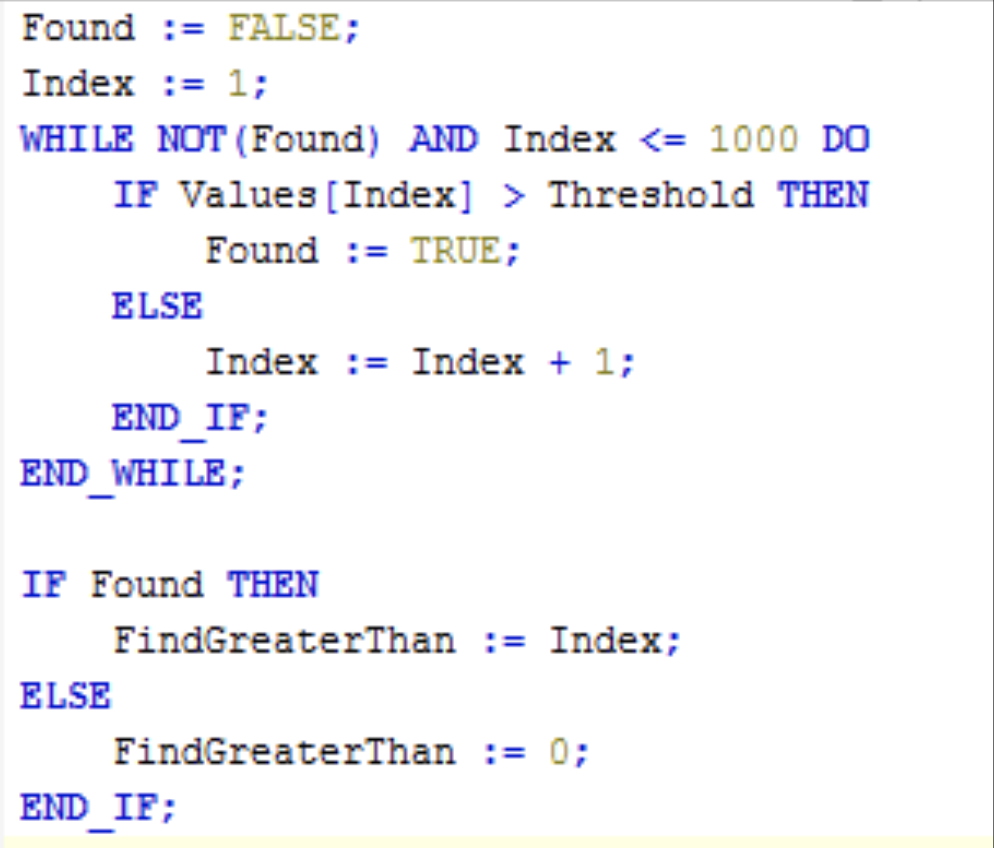
\includegraphics[width=0.8\textwidth]{./figures/st.png}
            {\footnotesize Source:~\url{http://www.contactandcoil.com/twincat-3-tutorial/structured-text/}}
        \end{column}
\end{columns}
\end{frame}

\section{Automated programming of PLCs}

\begin{frame}{Automated programming of PLCs}
\begin{itemize}
    \item The IEC 61131-3 languages are static in their programming.
    \item They are~\textbf{not} primarily designed for larger or dynamic systems.
    \item Modern software engineering methods like model-driven development are not natively supported.
    \item Rapid changes to the system become necessary.
    \item Validation and verification are crucial for automation systems.
\end{itemize}
$\Rightarrow$ Possible Solution: Programming methods that can \textbf{automatically} and \textbf{correctly} transform high-level specifications to low-level IEC 61131-3 code.
\end{frame}

\subsection{C/C++-based programming}

\begin{frame}{C/C++-based programming}
\begin{itemize}
	\item C/C++ are widespread systems programming languages.
    \item They allow access to low-level system operations (e.g. memory management).
    \item They support high-level abstractions (e.g. classes, modules).
	\item Widely used in micro controller programming.
    \item Currently two~\acrshort{acn:PLC} development environment allow for C/C++ POUs:
    \begin{itemize}
        \item Beckhoff TwinCAT3 
        \item B\&R Automation Studio
    \end{itemize}
    \item Both provide tools to ensure compliance with the~\acrshort{acn:PLC} execution semantics.
\end{itemize}
$\Rightarrow$ High-level programming is supported; Automatic generation of code or validation is not supported.
\end{frame}

\subsection{Formal description based}

\begin{frame}{Formal specification based}
\begin{itemize}
    \item Code generation from a formal specification.
    \item Allows for validation of the code against the specification.
    \item Design from a high-level abstraction of the control problem.
    \item Can either be model or non-model based.
    \item Widespread practice in software engineering or industrial plant design.
\end{itemize}
In the following section I present these formalizations:
\begin{itemize}
    \item Linear Temporal Logic
    \item UML/SysML
    \item Simulink
    \item PLCspecif
\end{itemize}
\end{frame}

\begin{frame}{Linear Temporal Logic}
\begin{itemize}
	\item Modal logic that allows to specify time based behavior.
    \item Conditions can be formalized over time constraints (e.g. something is true for all possible future states).
	\item Time is represented as a sequence of system states.
    \item \cite{Kuzmin:2013} use this to specify the controller behavior:
    \begin{itemize}
        \item Reactions to input changes are represented as LTL formula.
        \item Provides strong verification and validation methods.
        \item Not intuitive to use.
        \item Requires a deep understanding of modal logic.
    \end{itemize}
\end{itemize}

\begin{equation}
GX\left(V > \_V \rightarrow OldValCond \land FiringCond \land V := NewValExpr \right)
\label{eq:increase}
\end{equation}

\end{frame}

\begin{frame}{UML / SysML}
\begin{columns}
    \begin{column}{0.6\textwidth}
        \begin{itemize}
            \item \acrfull{acn:UML} and~\acrfull{acn:SysML} are widespread modeling languages.
            \item Several approaches use adapted state-charts and class-diagrams to model systems.
            \item \cite{WITSCH2015} and~\cite{VH:2014} define plcML.
            \begin{itemize}
                \item Allows to specify structure and behavior of the controller and its in-/outputs.
                \item Enables faster and more reliable controller development.
                \item The model can be translated into ST code.
            \end{itemize}
        \end{itemize}
    \end{column}
    \begin{column}{0.4\textwidth}
        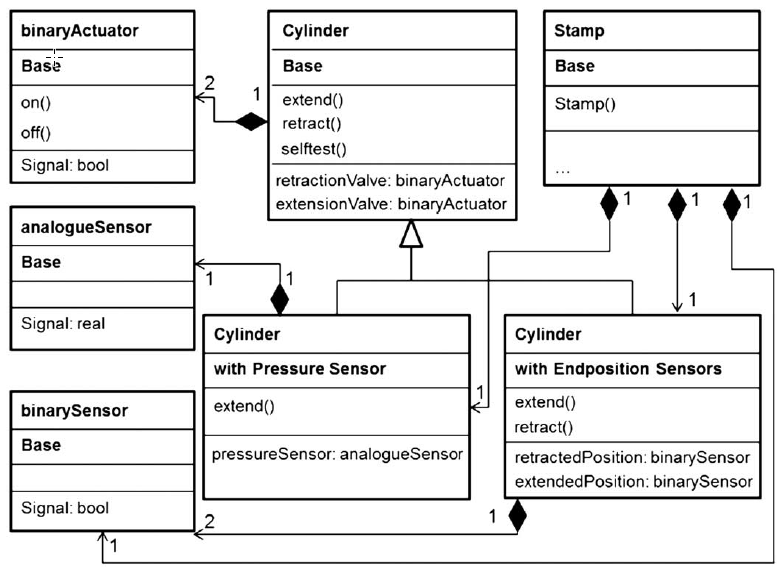
\includegraphics[width=\textwidth]{./figures/modAT4rMS_struct.png}
       {\footnotesize  Source:~\cite{VH:2014}}
    \end{column}
\end{columns}

\end{frame}

\begin{frame}{Simulink}
\begin{columns}
    \begin{column}{0.5\textwidth}
        \begin{itemize}
            \item Modeling software integrated into MathWorks MATLAB environment.
            \item Allows modeling and simulation of systems in multiple domains via toolboxes.
            \item Provide a coder that translates a model into ST code.
            \item \cite{7535242} extend this workflow with bound model checker verification.
            \item Easy to use method for designing large and complex systems.
        \end{itemize}
    \end{column}
    \begin{column}{0.5\textwidth}
        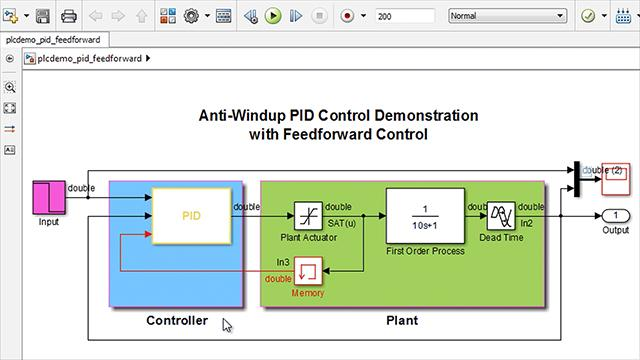
\includegraphics[width=\textwidth]{./figures/simulink.jpg}
       {\footnotesize  Source:~\url{https://de.mathworks.com/videos/simulink-plc-coder-overview-61206.html}}
    \end{column}
\end{columns}
\end{frame}

\begin{frame}{plcSpecif}
\begin{itemize}
    \item \cite{7819191} specify a custom graphical formalization language.
    \item It models systems with interacting modules.
    \item Modules consist of a structural and behavioral description.
    \item Behavior is represented as a mealy machine.
    \item They provide methods for formally verifying system properties.
    \item Additionally they focused on ease of use, traceability and readability.
    \item It is designed specifically for safety critical use cases.
\end{itemize}
\end{frame}

\section{Risks of automated programming}

\begin{frame}{Risks of automated programming}
\begin{itemize}
    \item \acrlong{acn:PLC} are often used in safety critical or real-time use cases.
    \item This requires a clear assessment of possible risks.
    \item Automatic generation of source code has inherent risks.
\end{itemize}
\pause
$\Rightarrow$ They need to be addressed before the system can be deployed.
\pause
Two components of the risk are addressed:
\begin{itemize}
    \item Transformation function correctness
    \item Runtime behavior guarantees
\end{itemize}
\end{frame}

\begin{frame}{Risks of automated programming}

\begin{block}{Transformation function correctness}
	\begin{itemize}
		\item Code generators have to ensure consistency between the code and modeled behavior.
		\item Must be specified and analyzed for every approach.
        \item Proof is often only given for common cases not all possible cases.
        \item Additionally traceability between the specification and the code should be possible.
	\end{itemize}
\end{block}
\pause
\begin{block}{Runtime guarantees}
    \begin{itemize}
        \item Behavior of the model on the actual~\acrshort{acn:PLC} has to be regarded.
        \item Transformations often use custom state machines that work over multiple PLC cycles.
        \item Validation methods have to ensure that the modeled behavior is consistent with the physical behavior.
    \end{itemize}
\end{block}
\end{frame}

\section{Conclusions}
\begin{frame}{Conclusions}

\begin{itemize}
    \item Modern automation systems require new programming methods.
    \pause
    \item Automated code generation from high-level abstractions is a viable options.
    \pause
    \item There are already well supported and capable approaches available (Simulink PLC coder, plcML)
    \begin{itemize}
        \item They are more effecitve and efficient as current approaches.
        \item They have high user acceptance and lower initial skill requirements.
    \end{itemize}
    \pause
    \item Efficient methods for risk analysis and validation on the deployment target are required.
\end{itemize}
\end{frame}

\begin{frame}
\vfill
\centering
{\LARGE Thank you for your attention.}\\
\vspace{1cm}
{\Large \textbf{Questions ?}}
\vfill
\end{frame}

\appendix
\beginbackup

\nocite{*}

\begin{frame}[allowframebreaks]{Glossaries}
\printglossaries
\end{frame}

\begin{frame}[allowframebreaks]{References}
\printbibliography
\end{frame}

\backupend

\end{document}
\grid
